\documentclass[10pt]{beamer}

\usepackage{polyglossia}
\usepackage{fontspec}
\usepackage{csquotes}
\usepackage{microtype}
\usepackage{color}
\usepackage{url}
\usepackage[backend=biber,style=iso-authoryear,sortlocale=cs_CZ,autolang=other,bibencoding=UTF8]{biblatex}
\usepackage{booktabs}
\usepackage{hyperref}
\usepackage{amsfonts}
\usepackage{amsthm}
\usepackage{amsmath}

\setdefaultlanguage{czech}
\setotherlanguage{english}
\setmainfont{TeX Gyre Termes}
\usetheme{Boadilla}
\usecolortheme{crane}
\setbeamertemplate{section in toc}[ball unnumbered]
\setbeamertemplate{bibliography item}{}
\addbibresource{zotero.bib}

\hypersetup{
	pdfencoding=auto,
	unicode=true,
	citecolor=green,
	filecolor=blue,
	linkcolor=red,
	urlcolor=blue
}

\makeatletter
\newcommand*{\currentSection}{\@currentlabelname}
\makeatother

\title[Hierarchické modely síťového provozu]
{
	Hierarchické modely síťového provozu
}

\titlegraphic
{
	
\includegraphics[width=0.2\columnwidth]{images/fjfi.png}
}

\author[Marek Dědič]
{
	Marek~Dědič\inst{1} \\
	Školitel:~Ing.~Tomáš~Pevný,~Ph.D.\inst{2}
}

\institute[FJFI ČVUT v Praze]
{
	\inst{1} ČVUT v Praze, Fakulta jaderná a fyzikálně inženýrská, Matematická informatika \and
	\inst{2} Cisco Systems Inc., Karlovo náměstí 10, Praha 2
}

\AtBeginSection[]{
	\begin{frame}{\currentSection}
		\tableofcontents[currentsection]
	\end{frame}
}

\begin{document}

\begin{frame}
	\titlepage
\end{frame}

\begin{frame}{Obsah}
	\tableofcontents
\end{frame}

\section{Motivace}
\begin{frame}{Motivace}
	\centering
	\textit{\enquote{100 percent of companies are calling malicious malware hosts}}\footnote{\cite{_cisco_2014}}
\end{frame}

\section{Řešená úloha}
\begin{frame}{Adresa URL}
	\centering
	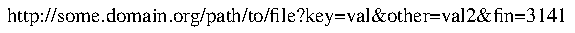
\includegraphics{images/url/url.pdf} \\
	\vspace{0.5cm}
	\pause
\includegraphics{images/url_legit/url_legit.pdf} \\
	\vspace{0.5cm}
	\pause
\includegraphics{images/url_malicious/url_malicious.pdf}\footnote{\only<3->{\cite{pevny_discriminative_2016}}}
\end{frame}

\begin{frame}[c]\frametitle{End--to--end učení}
	\centering
	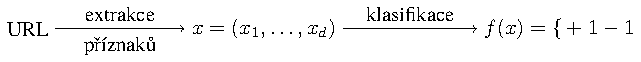
\includegraphics{images/end_to_end_learning/end_to_end_learning.pdf}
\end{frame}

\begin{frame}{Části a tokeny adresy URL}
	\centering
	
\includegraphics{images/url_subparts/url_subparts.pdf}
\end{frame}

\begin{frame}[c]\frametitle{Multi instanční učení}
	\centering
	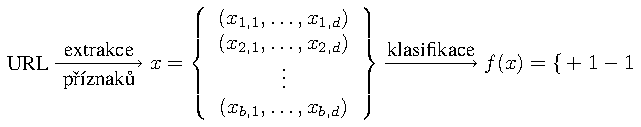
\includegraphics{images/multi_instance_learning/multi_instance_learning.pdf}
\end{frame}

\begin{frame}[c]\frametitle{Paradigma vloženého prostoru}
	\centering
	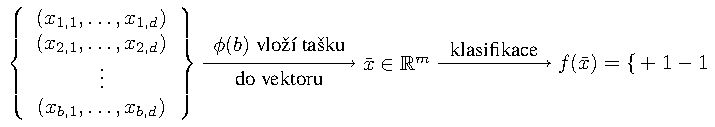
\includegraphics{images/embedded_space_paradigm/embedded_space_paradigm.pdf}
\end{frame}

\begin{frame}{Vkládající funkce \( \phi \)}
	\centering
	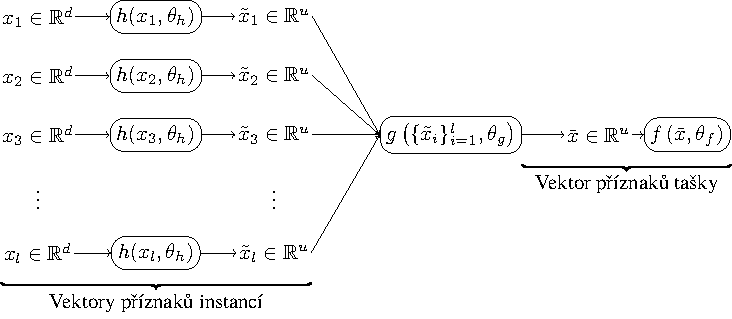
\includegraphics[width=0.9\pagewidth]{images/embedding_function/embedding_function.pdf}
\end{frame}

\begin{frame}{Můj model}
	\centering
	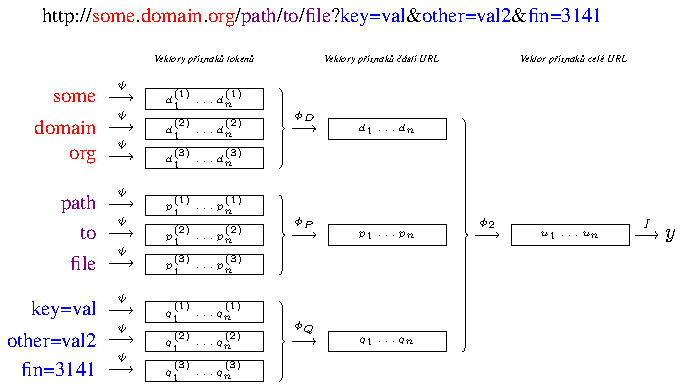
\includegraphics{images/model_modified_MIL/model_modified_MIL.pdf}
\end{frame}

\section{Výsledky mé práce}
\begin{frame}{Data}
	\centering
	\begin{tabular}{lrr}
		\toprule
		\null & \multicolumn{2}{c}{Počet adres} \\
		\cmidrule(l){2-3}
		Datový soubor & Legitimní & Malware \\
		\midrule
		Trénovací legitimní & 417 208 484 & 0 \\
		Trénovací směs & 17 390 889 & 34 359 733 \\
		Testovací legitimní & 1 522 255 052 & 0 \\
		Testovací směs & 2 855 992 & 4 051 944 \\
		\bottomrule
	\end{tabular}
\end{frame}

\begin{frame}{Výsledky mé práce}
	\centering
	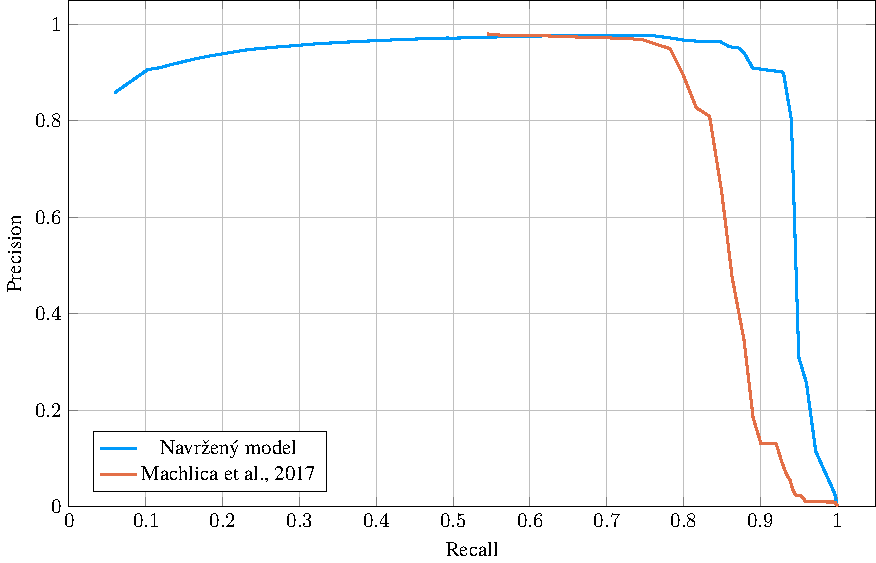
\includegraphics[width=0.9\columnwidth]{images/prior_art/prior_art.pdf}
	\nocite{machlica_learning_2017}
\end{frame}

\section{Závěr}
\newcommand{\ballotitem}{\item[\( \Box \)]}
\begin{frame}{Závěr}
	\begin{enumerate}
		\ballotitem Navržen model pro automatickou detekci malware ze síťového provozu
		\ballotitem Provedeno experimentální ověření navrženého modelu
		\ballotitem Navržený model dosahuje lepších výsledků než předchozí modely
		\ballotitem Klasifikátor s přesností i odezvou přesahující 90\%
	\end{enumerate}
\end{frame}

\begin{frame}{Další postup}
	\begin{enumerate}
		\ballotitem Opětovná aplikace multi-instančního přístupu pro modelování uživatelů
		\ballotitem Využití dalších polí HTTP hlavičky
		\ballotitem Využítí přenosových funkcí obsahujících šum
		\ballotitem Využití sebe-normalizujících neuronových sítí
		\ballotitem Využití techniky učení pomocí syntetických gradientů
	\end{enumerate}
\end{frame}

\begin{frame}{Seznam literatury}
	\printbibliography
\end{frame}

\begin{frame}{Dotazy}
	\begin{itemize}
		\item Byly během evaluace jednotlivé metody a jejich konfigurace porovnávány i z hlediska výpočetní náročnosti? Jaké jsou případně závěry z tohoto porovnání?
	\end{itemize}
\end{frame}

\end{document}
